\section{Arquitectura General}
\label{sec:diseno_estatico}

La plataforma adopta como guía de diseño la arquitectura hexagonal, cuyo objetivo central es aislar la lógica de negocio de los detalles técnicos externos: la base de datos, la interfaz de usuario o la comunicación con procesos auxiliares \parencite{martin_clean_architecture_2017}. A diferencia de una arquitectura en capas convencional, en la que las dependencias fluyen de arriba hacia abajo, este enfoque orienta todas las dependencias hacia el núcleo del sistema, de modo que los cambios tecnológicos no obliguen a modificar las reglas del negocio \parencite{evans_domain_driven_2003}.

La aplicación de este principio es pragmática y no estrictamente uniforme. El código Java se organiza en diez paquetes de primer nivel: \textit{backtesting}, \textit{market}, \textit{strategy}, \textit{trading}, \textit{training}, \textit{user}, \textit{wallet}, \textit{shared}, \textit{config} e \textit{interfaces}. Los siete primeros responden a capacidades funcionales del sistema; los tres últimos agrupan aspectos transversales. Dentro de los módulos más completos, como \textit{market}, \textit{strategy}, \textit{trading}, \textit{training}, \textit{user} y \textit{wallet}, se reconoce la separación entre dominio, aplicación e infraestructura de forma explícita. Esta organización proporciona el beneficio principal buscado: que la lógica financiera, el cálculo de beneficios y pérdidas, la gestión del libro mayor y la activación de estrategias puedan evolucionar con independencia de la base de datos, del motor de cálculo en Python o de la interfaz de usuario. La Figura~\ref{fig:arquitectura-hexagonal} ilustra de forma esquemática esta orientación.

\begin{figure}
    \centering
    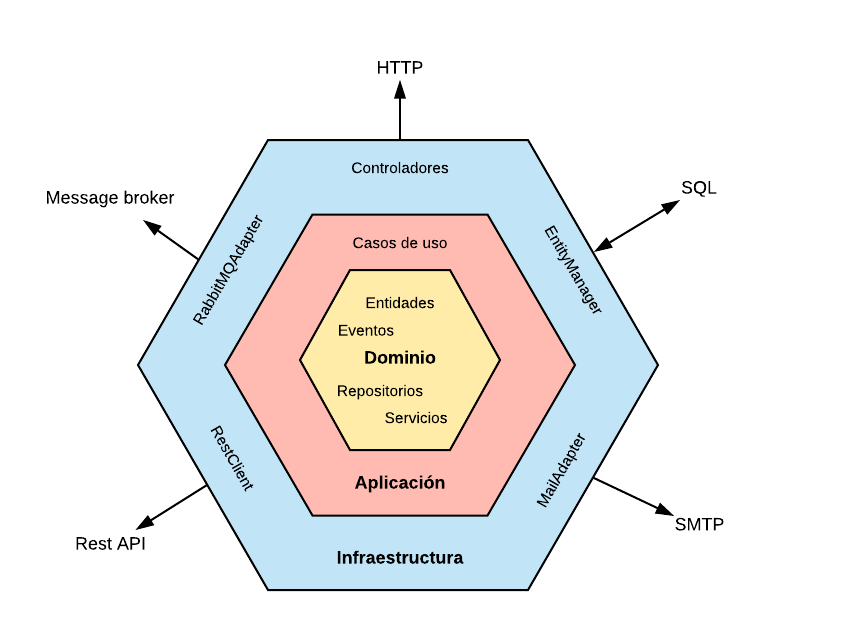
\includegraphics[width=0.8\textwidth]{Fotos/ArquitecturaHexagonal.png}
    \caption{Esquema conceptual de la orientación hexagonal del proyecto; no representa literalmente toda la jerarquía de paquetes.}
    \label{fig:arquitectura-hexagonal}
\end{figure}

\subsection{Estructura y componentes del sistema}

\subsubsection{Módulos del backend Java}

La base compartida de todo el sistema reside en el paquete \textit{shared}. La clase abstracta \textit{BaseEntity} dota a todas las entidades de la base de datos de tres campos estandarizados: un identificador autogenerado, una marca de tiempo de creación y un indicador de borrado lógico. El uso de borrado lógico en lugar de eliminación física garantiza la trazabilidad histórica de todas las operaciones: cualquier baja se expresa como una actualización de estado sin destruir el registro original \parencite{fowler_patterns_2002}. En un sistema contable, responder a qué capital tenía una estrategia al detenerse o por qué fue cerrada una posición es un requisito del dominio, no una conveniencia de implementación.

El módulo de \textbf{trading en tiempo real} es el núcleo operativo del sistema. La entidad \textit{InstanciaEstrategia} modela una configuración activa de ejecución: almacena el nombre de la estrategia, el capital asignado con precisión decimal, los parámetros de riesgo y el estado de ciclo de vida, que puede ser activa, detenida o terminada. \textit{Posicion} representa una operación de mercado individual, registrando el símbolo negociado, el precio de entrada exacto y un indicador de posición abierta que el motor consulta para evitar órdenes duplicadas sobre el mismo par. El historial financiero se construye con \textit{LedgerEntry}, un registro inmutable de cada movimiento de capital cuyo tipo se expresa mediante \textit{LedgerType}, que cubre ocho situaciones posibles: capital disponible, reservado, comprometido, margen comprometido, beneficio realizado, beneficio no realizado, comisión y estrategia pausada. La cartera digital implementa un doble saldo, formado por el balance real y el balance disponible, que impide sobregiros cuando varias estrategias compiten simultáneamente por el mismo capital. En la capa de aplicación, \textit{PaperTradingService} simula la ejecución de órdenes y valida las reglas de riesgo, mientras que \textit{AccountingService} actúa como único responsable de todas las operaciones monetarias, operando siempre con bloqueos de escritura para garantizar consistencia \parencite{goetz_java_concurrency_2006}. \textit{StrategyRuntimeCoordinator} gestiona el ciclo de vida de los procesos Python de trading mediante un grupo de hilos virtuales de la JDK 21 \parencite{goetz_jep444_2023}, lo que permite lanzar una instancia por estrategia activa sin saturar el grupo de hilos del sistema operativo y manteniendo un modelo de programación secuencial idiomático \parencite{goetz_java_concurrency_2006}.

La robustez financiera del sistema descansa en tres garantías transaccionales complementarias. Los repositorios de cartera digital e instancia de estrategia aplican bloqueos pesimistas de escritura exclusiva, impidiendo que dos hilos modifiquen el mismo saldo de forma simultánea y evitando así las inconsistencias contables que pueden surgir en escenarios de ejecución concurrente \parencite{goetz_java_concurrency_2006,oracle_mysql_acid_2024}. Todos los movimientos monetarios pasan obligatoriamente por \textit{AccountingService}, que los envuelve en transacciones atómicas con garantía de reversión completa ante cualquier fallo: si algún paso falla, el balance real, el balance disponible y el libro mayor vuelven al estado anterior sin dejar registros parciales \parencite{spring_data_jpa_2024,kleppmann_designing_2017}. El libro mayor actúa además como registro de auditoría permanente: dado que sus entradas son inmutables, es posible reconstruir el estado financiero de cualquier cartera en cualquier instante histórico, lo que facilita la verificación de discrepancias \parencite{lopez_de_prado_advances_2018,fowler_patterns_2002}.

El módulo de \textbf{backtesting} permite validar el comportamiento de una estrategia sobre datos reales sin riesgo financiero \parencite{pardo_evaluation_2008}. La entidad \textit{Vela} almacena los datos de precio y volumen con precisión decimal de ocho cifras y marca temporal en milisegundos. \textit{VelaDTO} emplea cadenas de texto para los precios al deserializar desde la interfaz de Binance, evitando pérdidas de precisión numérica durante la transferencia. \textit{BacktestingService} recupera las velas, serializa el mensaje en el formato binario del protocolo y lo envía al motor Python; a continuación, recibe los resultados estadísticos (tasa de acierto, factor de ganancia, caída máxima y ratio de Sharpe) y los persiste en un archivo de valores separados por comas.

El módulo de \textbf{descarga de datos de mercado} cubre el flujo de extracción, transformación y carga de datos históricos. \textit{FetchService} implementa la sincronización incremental: consulta la última vela almacenada y solicita a Binance únicamente los datos nuevos, persistiéndolos en lotes mediante inserciones masivas nativas \parencite{oracle_mysql_insert_opt_2024}, pues la sobrecarga de seguimiento de contexto del mapeador objeto-relacional resulta inasumible a ese volumen en tiempo interactivo; la sentencia condicional de actualización garantiza además la idempotencia de las descargas repetidas y repara automáticamente huecos que pudieran haber quedado por desconexiones o cambios de interfaz, resincronizando desde el punto de ruptura sin necesidad de intervención manual \parencite{kimball_data_2004,pardo_evaluation_2008}. El motor Python gestiona el acceso a la interfaz de Binance respetando sus límites de tasa mediante dos estrategias complementarias: de forma proactiva, introduce pausas entre peticiones según los umbrales conocidos de la interfaz; de forma reactiva, interpreta los códigos de respuesta 429 y 418 aplicando retroceso exponencial con reintentos automáticos \parencite{binance_rate_limits_2024,kleppmann_designing_2017}. \textit{MarketDataService} orquesta en una sola llamada la descarga y el cálculo de indicadores. \textit{IndicatorsService} delega el cálculo al motor Python y persiste los resultados como entidades de indicador técnico.

El módulo de \textbf{inteligencia artificial y optimización} gestiona el entrenamiento supervisado y la búsqueda de la configuración óptima de los modelos. \textit{AITrainingService} prepara el conjunto de datos, selecciona el tipo de modelo y lo envía al motor Python, recibiendo a cambio las métricas de evaluación. \textit{AIOptimizationService} extiende ese flujo incorporando parámetros de búsqueda como el número de ensayos y el umbral mínimo de exactitud aceptable, delegando al motor la búsqueda bayesiana mediante Optuna \parencite{feurer_hyperparameter_2019}.

El módulo de \textbf{gestión de usuarios y carteras digitales} implementa el acceso a la plataforma con las garantías de seguridad propias del software financiero \parencite{owasp_password_2024}. \textit{Usuario} es una clase Java sin dependencias de infraestructura: su persistencia se delega a un adaptador que traduce entre la representación de dominio y la entidad de base de datos mediante un mapeador dedicado. \textit{UsuarioApplicationService} implementa los casos de uso de creación y autenticación de usuarios, aplicando cifrado de contraseña con BCrypt \parencite{provos_bcrypt_1999}: un algoritmo adaptativo que incorpora una sal aleatoria por usuario, de modo que las contraseñas nunca se almacenan en texto plano y la dificultad de cómputo puede endurecerse sin modificar el esquema de datos. Las credenciales de acceso a la base de datos se inyectan en tiempo de arranque mediante variables de entorno cargadas desde un archivo local excluido del control de versiones; si alguna variable obligatoria está ausente, la aplicación falla de forma inmediata y visible en lugar de propagarse como un error silencioso en ejecución \parencite{kleppmann_designing_2017}. \textit{WalletService} gestiona la creación y consulta de carteras en modo de operativa simulada. \textit{SessionManager} mantiene en memoria el usuario autenticado activo, restringe el acceso a cualquier operación sensible a sesiones previamente autenticadas y registra un gancho de cierre que detiene todas las estrategias activas al apagar la aplicación \parencite{gamma_design_1994}.

Entre las utilidades transversales, \textit{PathConfig} centraliza la resolución de rutas del sistema de archivos con independencia del directorio desde el que se ejecute la aplicación; \textit{AppConstants} define las constantes del contrato entre Java y Python, como claves de objetos serializados y cabeceras de archivos; y \textit{IpcMessagePackCodec} implementa el protocolo binario de bajo nivel, encapsulado en un registro inmutable con versión de protocolo, tipo de mensaje, identificador de correlación y contenido.

\subsubsection{Patrones de diseño aplicados}
\label{sec:patrones}

La arquitectura hace uso explícito de varios patrones de diseño reconocibles en puntos concretos del código \parencite{gamma_design_1994,fowler_patterns_2002}. El patrón \textbf{Repositorio} aparece en todas las interfaces de acceso a datos, como \textit{LedgerRepository} o \textit{WalletRepository}, abstrayendo los detalles de consulta y persistencia frente a los servicios de aplicación. El patrón \textbf{Comando} está presente tanto en el gestor principal de la interfaz de línea de comandos como en cada clase de comando individual, que encapsula la lógica de una acción y delega su ejecución al servicio de aplicación correspondiente. El patrón \textbf{Fachada} se aplica en \textit{PythonBridgeFacade}, que simplifica la interacción con los procesos Python detrás de una interfaz uniforme, ocultando los detalles del protocolo binario a los servicios que lo usan. El patrón \textbf{Constructor} se utiliza en \textit{PythonBridgeRequest} para configurar cada invocación al motor Python de forma legible y sin constructores de múltiples parámetros. El patrón \textbf{Registro único} aparece en \textit{SessionManager} gestionado por Spring, garantizando que solo exista una sesión activa en todo momento. Por último, en el motor Python, la jerarquía basada en \textit{BaseStrategy} introduce el patrón \textbf{Estrategia}: cada implementación concreta define los mismos tres métodos obligatorios sin modificar el motor de ejecución \parencite{gamma_design_1994}.

\subsubsection{Motor Python}

Java actúa como orquestador del sistema por su tipado estático, soporte transaccional ACID y modelo de concurrencia basado en hilos virtuales \parencite{goetz_java_concurrency_2006}; Python se incorpora como motor de cálculo por disponer del ecosistema de análisis de datos y aprendizaje automático más maduro del mercado \parencite{hilpisch_python_2018,goodfellow_deep_2016}. El subsistema Python tiene una estructura intencionalmente sencilla. Se organiza en una única carpeta de scripts, donde cada archivo corresponde a un motor que se ejecuta como un proceso independiente invocado por el orquestador Java. Los motores disponibles cubren las siguientes funciones: descarga de velas de Binance, cálculo de indicadores técnicos, simulación histórica de estrategias, trading en tiempo real con reglas clásicas, trading en tiempo real con modelo neuronal, entrenamiento supervisado y optimización de configuraciones. Todos comparten un módulo de utilidades comunes y el módulo del protocolo de comunicación. La carpeta de estrategias, separada de los motores, contiene la clase base abstracta \textit{BaseStrategy} y las implementaciones concretas. Esta separación garantiza que añadir una nueva estrategia no requiera modificar ningún motor existente. La descarga de datos históricos aprovecha además la concurrencia de Python mediante un grupo de hilos que lanza múltiples peticiones simultáneas a la interfaz de Binance, reduciendo significativamente el tiempo total de descarga cuando se solicitan varios periodos o símbolos a la vez \parencite{python_concurrent_futures_2024,binance_rest_api_2024}.

\subsection{Comunicación entre procesos}
\label{sec:ipc}

La comunicación entre el orquestador Java y los motores Python es un componente crítico de la arquitectura. Se ha definido un protocolo versionado de forma explícita para garantizar compatibilidad y permitir su evolución sin romper el funcionamiento existente \parencite{richards_software_2022}.

Todo mensaje intercambiado respeta una estructura envolvente con cuatro campos: la versión del protocolo, el tipo de mensaje como código semántico de la operación (solicitud de descarga, respuesta de indicadores, error, señal en tiempo real, entre otros), un identificador de correlación único por petición para asociar solicitudes y respuestas \parencite{hohpe_enterprise_2003}, y el contenido específico de la operación en formato binario. Para evitar problemas de sincronización en las tuberías de comunicación, cada mensaje va precedido de un entero de cuatro bytes en orden de red que especifica la longitud exacta del cuerpo. El contenido se serializa en \textbf{MessagePack} \parencite{furuhashi_msgpack_2013}, un formato binario más compacto que su equivalente en texto plano y sin pérdida de compatibilidad de tipos \parencite{kleppmann_designing_2017}. El volumen de datos intercambiados por sesión puede alcanzar cientos de miles de velas con sus indicadores calculados, lo que convierte la eficiencia de serialización en un requisito práctico; el prefijo de longitud de cuatro bytes simplifica además la lectura del flujo sin necesidad de delimitadores en el contenido.

La comunicación utiliza la salida estándar como canal exclusivo para el flujo de mensajes binarios, mientras que los registros y errores se envían por el canal de error estándar, garantizando que el orquestador lea el flujo de datos sin interferencias \parencite{newman_building_2015}. Para el trading en tiempo real, el motor Python emite líneas de control con un prefijo de señal seguidas del contenido de la orden en formato estructurado. El coordinador Java lee cada línea y delega en el analizador de protocolo para identificar las señales; una vez reconocidas, las entrega al servicio de operativa simulada para su procesamiento contable.

La convención de códigos de salida permite al orquestador tomar decisiones de recuperación de forma automatizada \parencite{richards_software_2022}: el código cero indica ejecución exitosa; el uno señala un error de lógica no recuperable sin intervención del usuario, como una estrategia inválida o un modelo no entrenado; el dos corresponde a un error en los datos de entrada; y el tres indica una interrupción por tiempo de espera agotado o cierre externo del proceso.

Para evitar que procesos bloqueados consuman recursos indefinidamente, se definen tiempos de espera diferenciados según la operación \parencite{kleppmann_designing_2017}: 120 segundos para el arranque del proceso, que incluye la importación de bibliotecas pesadas como TensorFlow; 300 segundos de inactividad máxima para operaciones de descarga o cálculo de indicadores; 900 segundos para la simulación histórica, aunque el caso típico concluye en menos de un minuto \parencite{pardo_evaluation_2008}; 1800 segundos para el entrenamiento de modelos, que puede incluir validación cruzada sobre series temporales \parencite{lopez_de_prado_advances_2018}; y 3600 segundos para la optimización de hiperparámetros, cuya duración puede prolongarse en función del espacio de búsqueda definido. Si un proceso supera alguno de estos umbrales sin producir actividad, el orquestador lo termina forzosamente y lo registra con el código de salida tres.

\subsection{Ventajas y desventajas de la arquitectura}

La adopción de este esquema responde a una evaluación de sus beneficios frente a las necesidades del sistema \parencite{treleaven_algorithmic_2013}.

Entre las ventajas, la más relevante es la \textbf{mantenibilidad}. Si fuera necesario cambiar el motor de base de datos de MySQL a otro sistema, solo se vería afectado el adaptador de persistencia; la lógica de las estrategias en Python y los servicios Java permanecerían intactos \parencite{spring_data_jpa_2024,martin_clean_architecture_2017}. Una consecuencia directa de esa separación es la \textbf{facilidad para escribir pruebas}: los servicios de aplicación dependen de interfaces y no de implementaciones concretas, lo que permite verificar la lógica de contabilidad sin necesidad de lanzar los procesos de inteligencia artificial ni conectarse a la base de datos real \parencite{martin_clean_architecture_2017,evans_domain_driven_2003}. Finalmente, la \textbf{independencia entre subsistemas} permite trabajar de forma aislada en la robustez del orquestador Java mientras se perfeccionan los modelos matemáticos en Python, siempre que el contrato de datos entre ambas partes se mantenga constante \parencite{hilpisch_python_2018,newman_building_2015}.

Entre las limitaciones, la principal es el \textbf{volumen de código adicional}. El flujo de datos requiere transformar entidades en objetos de transferencia al pasar de una capa a otra, lo que incrementa el código necesario frente a una arquitectura más directa \parencite{richards_software_2022,martin_clean_architecture_2017}. Esta limitación se mitiga mediante el uso de Lombok para la generación automática de constructores y mapeadores dedicados \parencite{lombok_project_2024}. La otra limitación es la \textbf{latencia acumulada}: en sistemas de trading de altísima frecuencia, el paso de información a través de múltiples capas puede introducir pequeños retardos \parencite{treleaven_algorithmic_2013}. Para los intervalos de tiempo gestionados en este proyecto, velas de un minuto o superiores, este impacto es despreciable frente a la seguridad transaccional obtenida \parencite{oracle_mysql_acid_2024,pardo_evaluation_2008}.